%%%%%%%%%%%%%%%%%%%%%%%%%%%%%%%%%%%%%%%%%
% Short Sectioned Assignment
% LaTeX Template
% Version 1.0 (5/5/12)
%
% This template has been downloaded from:
% http://www.LaTeXTemplates.com
%
% Original author:
% Frits Wenneker (http://www.howtotex.com)
%
% License:
% CC BY-NC-SA 3.0 (http://creativecommons.org/licenses/by-nc-sa/3.0/)
%
%%%%%%%%%%%%%%%%%%%%%%%%%%%%%%%%%%%%%%%%%

%----------------------------------------------------------------------------------------
%	PACKAGES AND OTHER DOCUMENT CONFIGURATIONS
%----------------------------------------------------------------------------------------

\documentclass[paper=a4, fontsize=11pt]{scrartcl} % A4 paper and 11pt font size

\usepackage[T1]{fontenc} % Use 8-bit encoding that has 256 glyphs
\usepackage{fourier} % Use the Adobe Utopia font for the document - comment this line to return to the LaTeX default
\usepackage[english]{babel} % English language/hyphenation
\usepackage{amsmath,amsfonts,amsthm} % Math packages
\usepackage{graphicx}  

\usepackage{lipsum} % Used for inserting dummy 'Lorem ipsum' text into the template

\usepackage{sectsty} % Allows customizing section commands
\allsectionsfont{\centering \normalfont\scshape} % Make all sections centered, the default font and small caps

\usepackage{fancyhdr} % Custom headers and footers
\pagestyle{fancyplain} % Makes all pages in the document conform to the custom headers and footers
\fancyhead{} % No page header - if you want one, create it in the same way as the footers below
\fancyfoot[L]{} % Empty left footer
\fancyfoot[C]{} % Empty center footer
\fancyfoot[R]{\thepage} % Page numbering for right footer
\renewcommand{\headrulewidth}{0pt} % Remove header underlines
\renewcommand{\footrulewidth}{0pt} % Remove footer underlines
\setlength{\headheight}{13.6pt} % Customize the height of the header

\numberwithin{equation}{section} % Number equations within sections (i.e. 1.1, 1.2, 2.1, 2.2 instead of 1, 2, 3, 4)
\numberwithin{figure}{section} % Number figures within sections (i.e. 1.1, 1.2, 2.1, 2.2 instead of 1, 2, 3, 4)
\numberwithin{table}{section} % Number tables within sections (i.e. 1.1, 1.2, 2.1, 2.2 instead of 1, 2, 3, 4)

\setlength\parindent{0pt} % Removes all indentation from paragraphs - comment this line for an assignment with lots of text

%----------------------------------------------------------------------------------------
%	TITLE SECTION
%----------------------------------------------------------------------------------------

\newcommand{\horrule}[1]{\rule{\linewidth}{#1}} % Create horizontal rule command with 1 argument of height

\title{	
\normalfont \normalsize 
\textsc{ETH Zurich, IDSC} \\ [25pt] % Your university, school and/or department name(s)
\horrule{0.5pt} \\[0.4cm] % Thin top horizontal rule
\huge Car model Equations \\ % The assignment title
\horrule{2pt} \\[0.5cm] % Thick bottom horizontal rule
}

\author{Edo Jelavic} % Your name

\date{\normalsize\today} % Today's date or a custom date

\begin{document}

\maketitle % Print the title



\section{Four Wheeled Car Model} \label{FourWheelModel}

Four wheeled car model is built upon the schematic depicted in \ref{4wheelCar}.

\begin{figure}[h!]
	\centering
	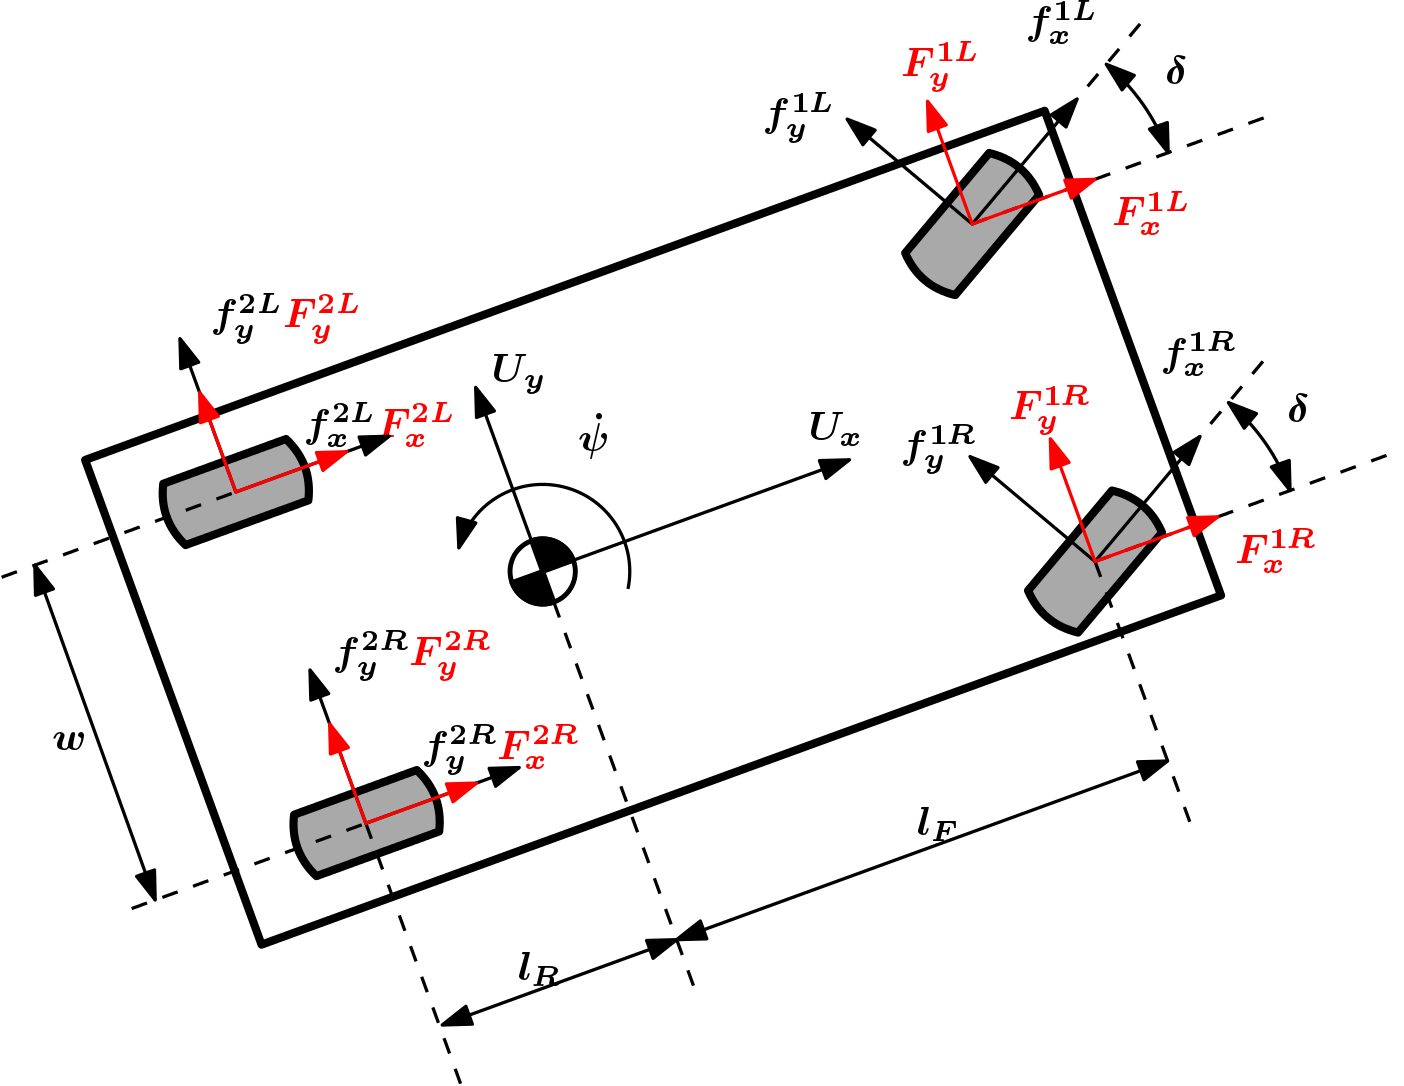
\includegraphics[width=0.6\textwidth]{drawings/4wheelCar.png}
	\caption{4 wheeled car model}
	\label{4wheelCar}
\end{figure}

In Figure \ref{4wheelCar}, superscript $1L$ refers to the front left wheel, $1R$ refers to front right wheel and similarly $2L$ and $2R$ refer to rear left and right wheel, respectively. Subscripts $x$ and $y$ refer to longitudinal or lateral forces. Capital letter $F$ denotes a force that is tied to the car coordinate frame (red frames and forces painted red in Figure \ref{4wheelCar}) while the lower case letters $f$ denote forces in the tire coordinate frame. Four wheeled model is described by following equations:

\begin{align}
\dot{{U_x}} &  = \frac{1}{m} \left( F_x^{1L} + F_x^{1R} + F_x^{2L} +F_x^{2R} \right) + U_yr \label{4wheelCarEq1}      \\
\dot{U_y}   & = \frac{1}{m} \left(F_y^{1L} + F_y^{1R} + F_y^{2L} + F_y^{2R}  \right)  - U_xr \\
\dot{r}  & = \frac{1}{I_z}  \left( l_F \left(F_y^{1L} + F_y^{1R} \right) -l_R \left(F_y^{2L} + F_y^{2R} \right) + \frac{w}{2}\left(F_x^{1R} + F_x^{2R} - F_x^{1L} - F_x^{2L} \right)    \right) \\
\dot{\psi}  & = r \\
\dot{x}  & = U_x\cos\psi - U_y\sin\psi \\
\dot{y}  & = U_x\sin\psi + U_y\cos\psi \\
\dot{\omega}^{1L}  & = \frac{1}{I_{\omega}}\left( \hat{T}^{1L} - f_x^{1L}R\right)  \\
\dot{\omega}^{1R}  & = \frac{1}{I_{\omega}}\left( \hat{T}^{1R} - f_x^{1R}R\right) \\ 
\dot{\omega}^{2L}  & = \frac{1}{I_{\omega}}\left( \hat{T}^{2L} - f_x^{2L}R\right)  \\
\dot{\omega}^{2R}  & = \frac{1}{I_{\omega}}\left( \hat{T}^{2R} - f_x^{2R}R\right) \label{4wheelCarEq10} \\ 
\hat{T}^j& = \begin{cases}   T^j, \qquad \omega^j > 0 \\
f_x^jR, \qquad \omega^j = 0 
\end{cases}, \text{ where } \quad j \in \{1L, 1R, 2L, 2R \} \label{discontinuous}
\end{align}

In equations \ref{4wheelCarEq1} - \ref{4wheelCarEq10} $w$ denotes width of the car. Superscript $1$ denotes the front wheel and superscript $2$ denotes the rear wheel. Subscript $x$ denotes longitudinal direction and subscript $y$ denotes lateral direction. For example, $f^1_x$ is a force on the front tire in the longitudinal direction (in the tire frame). $U_x$ and $U_y$ denote longitudinal and lateral velocities of the car, respectively. Yaw rate is denoted with $r$ and $\psi$ is the yaw angle (or heading angle). 
$m$ is a mass of the car.
$I_z$ is a moment of inertia around the z-axis.
$I_\omega$ is the wheel moment of inertia around axis of rotation of wheel.
$l_F$ is a distance between Center of Gravity (COG) and the front axle, $l_R$ is the distance between COG and the rear axle. $w$ is the distance from left to the right wheel. $R$ is the radius of the wheels. The rotational velocity of the wheels is denoted with $\omega$ and $\mu$ is a friction coefficient between the tire and the surface. Steering angle is denoted with $\delta$ and $T$ denotes torque applied to the wheels (those are inputs into the system). Lateral and longitudinal forces in the tire frame are calculated as follows:

\begin{align}
\mu^j & =D\sin(C\arctan(Bs^j)) \label{4wheelPacejkaEq1}  \\
\mu_i^j & = -\frac{s_i^j}{s^j}\mu^j   \\
f_i^j & = \mu f_{z}^j \mu_i^j \label{lateralLongitudinal}  \\
s_x^j & = \frac{v_x^j - \omega^jR}{\omega^jR}   \\
s_y^j & = \left( 1 + s_x^j\right) \frac{v_y^j}{v_x^j}  \\ 
s^j & = \sqrt{ (s_x^j)^2 + (s_y^j)^2 }   \\
where \quad &  i \in\left\{ {x, y}\right\}, j \in \left\{ {1L,1R,2L, 2R}\right\} \label{4wheelPacejkaEq6}
\end{align}

Relationship between forces in the car frame (red frame in Figure \ref{4wheelCar}) and forces in the tire frame is given by:

\begin{align}
\begin{bmatrix}
F^j_x  \label{forcesConversion1}\\
F^j_y
\end{bmatrix} & = \begin{bmatrix}
\cos\delta & -\sin\delta \\
\sin\delta & \cos\delta
\end{bmatrix} \begin{bmatrix}
f^j_x \\
f^j_y
\end{bmatrix}
\text{where}  \quad j \in \left\{ {1L,1R}\right\} \\
\begin{bmatrix}
F^j_x \\
F^j_y
\end{bmatrix} & = \begin{bmatrix}
f^j_x \\
f^j_y
\end{bmatrix}
\text{where}  \quad j \in \left\{ {2L,2R}\right\} \label{forcesConversion3} \\
\end{align}

Similar relations hold for velocities as well:

\begin{align}
\begin{bmatrix}
v^{1L}_x \\
v^{1L}_y
\end{bmatrix} & = \begin{bmatrix}
\cos\delta & \sin\delta \\
-\sin\delta & \cos\delta
\end{bmatrix} \begin{bmatrix}
U_x - r\frac{w}{2} \\
U_y + r l_F
\end{bmatrix} \\
\begin{bmatrix}
v^{1R}_x \\
v^{1R}_y
\end{bmatrix} & = \begin{bmatrix}
\cos\delta & \sin\delta \\
-\sin\delta & \cos\delta
\end{bmatrix} \begin{bmatrix}
U_x + r\frac{w}{2} \\
U_y + r l_F
\end{bmatrix} \\
\begin{bmatrix}
v^{2L}_x \\
v^{2L}_y
\end{bmatrix} & = \begin{bmatrix}
U_x - r\frac{w}{2} \\
U_y - r l_R
\end{bmatrix}\\
\begin{bmatrix}
v^{2R}_x \\
v^{2R}_y
\end{bmatrix} & = \begin{bmatrix}
U_x + r\frac{w}{2} \\
U_y - r l_R
\end{bmatrix}
\end{align}

Still missing, are the expressions for computing vertical forces $F^j_z$ (note that $F^j_z = f^j_z$). To obtain expressions for these forces a weight transfer model has to be derived. It all starts by looking at the car confined to the $y-z$ plane. Rear view of the car in the $y-z$ plane is shown in Figure \ref{4wheelYZplane}.

\begin{figure}[h!]
	\centering
	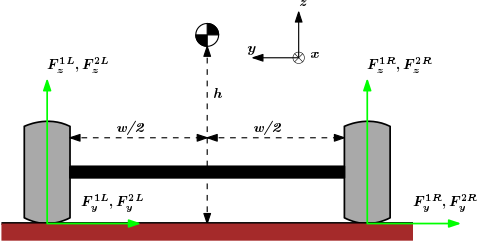
\includegraphics[width=0.7\textwidth]{drawings/4wheelYZplane.png}
	\caption{4 wheeled car model, back view}
	\label{4wheelYZplane}
\end{figure}

Looking at the Figure \ref{4wheelYZplane} one obtains the first equation of four equations in total. The first equation is expressed in the equation \ref{YZtorqueBalance}; it is merely a balance of torques around the center of gravity. $h$ denotes the distance between COG and the ground.

\begin{equation}
\left(F^{1L}_z+F^{2L}_z \right)\frac{w}{2} + h\left(F^{1L}_y + F^{1R}_y + F^{2L}_y + F^{2R}_y \right) = \left(F^{1R}_z+F^{2R}_z \right)\frac{w}{2} \label{XZtorqueBalance}
\end{equation} 

Second equation is obtained by looking at the torque balance in $x-z$ plane. Side view of the car is shown in Figure \ref{4wheelXZplane}.

\begin{figure}[h!]
	\centering
	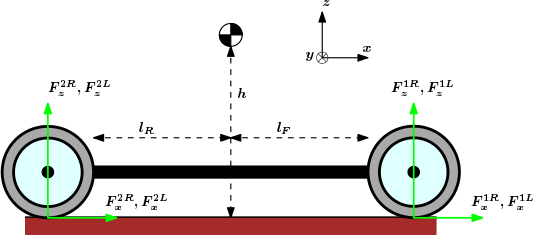
\includegraphics[width=0.7\textwidth]{drawings/4wheelXZplane.png}
	\caption{4 wheeled car model, side view}
	\label{4wheelXZplane}
\end{figure}

Equation of torque balance in $x-z$ plane is given by:

\begin{equation}
\left(F^{2R}_z+F^{2L}_z \right)l_R + h\left(F^{1L}_x + F^{1R}_x + F^{2L}_x + F^{2R}_x\right) = \left(F^{1R}_z+F^{1L}_z \right)l_F \label{YZtorqueBalance}
\end{equation}

The third equation is given by:

\begin{equation}
F^{1L}_z+F^{1R}_z + F^{2L}_z + F^{2R}_z = mg\label{gravityBalance}
\end{equation} 

Where $m$ is mass and $g$ is gravitational acceleration. Finally, the last equation arises from geometrical considerations. In Figure \ref{deflectedPlane}, a deflected $x-y$ plane is shown. It is assumed that all the rotations happen around the COG.

\begin{figure}[h!]
	\centering
	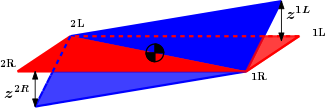
\includegraphics[width=0.7\textwidth]{drawings/deflectedPlane.png}
	\caption{4 wheeled car model, deflected $x-y$ plane amid weight transfer}
	\label{deflectedPlane}
\end{figure}

From Figure \ref{deflectedPlane} it can be seen that deflection on the wheel $2R$ has to be equal to the deflection at the diagonally opposite wheel $1L$. Hence, for the deflections $z$, it has to hold:

\begin{align}
z^{1L} + z^{2R} &= 0 \label{deflections1}\\
z^{1R} + z^{2L} &= 0 \label{deflections2}
\end{align}

If one sums up the equations \ref{deflections1} and \ref{deflections2}, one obtains:

\begin{equation}
z^{1L} + z^{2R} = z^{1R} + z^{2L} \label{deflections} 
\end{equation}

It is assumed that there is a spring on each wheel. Therefore, the following equation holds:

\begin{equation}
F^j_z =c^jz^j, where \quad j \in \{1L,1R,2L,2R \} \label{spring} 
\end{equation}

In equation \ref{spring}, $z$ are deflections and $c$ are spring constants. Combining equations \ref{spring} and \ref{deflections} and using a simplification $c^i = c^j, \forall i,j \in \{1L,1R,2L,2R \}$, one gets the fourth equation:

\begin{equation}
F_z^{1L} + F_z^{2R} = F_z^{1R} + F_z^{2L} \label{forcesBalance} 
\end{equation}

By plugging in the expressions for lateral and longitudinal forces ($F_x$, $F_y$) from equation \ref{lateralLongitudinal} and equations \ref{forcesConversion1} - \ref{forcesConversion3}  into equations \ref{YZtorqueBalance}, \ref{XZtorqueBalance}, \ref{gravityBalance} and \ref{forcesBalance}, one obtains expressions for vertical forces $F_z$. These are given by the following set of equations:

\begin{align}
F^{1L}_z &= mg\frac{BG - CF + BH - DF - CH + DG}{den} \\
F^{1R}_z &= mg\frac{AG - EC + AH - ED + CH - DG}{den} \\
F^{2L}_z &= mg\frac{AF - EB + AH - ED + BH - DF}{den} \\
F^{1R}_z &= mg\frac{AF - EB - AG + EC - BG + CF}{den}
\end{align}

where:

\begin{align}
den &= 2(AF - EB - AG + EC + BH - DF - CH + DG) \\
A &= -\frac{w}{2} - C_1 - C_2 \\
B &= \frac{w}{2} - C_3 - C_4 \\
C &= -\frac{w}{2} - C_5 \\
D &= \frac{w}{2} - C_6 \\
E &= K_1 - K_2 - l_F \\
F &= K_3 - K_4 - l_F \\
G &= K_5 + l_R \\
H &= K_6 + l_R \\
C_1 &= -\mu \mu^{1L}_x h \sin(\delta) \\
C_2 &= -\mu \mu^{1L}_y h \cos(\delta) \\
C_3 &= -\mu \mu^{1R}_x h \sin(\delta) \\
C_4 &= -\mu \mu^{1R}_y h \cos(\delta) \\
C_5 &= -\mu \mu^{2L}_y h  \\
C_6 &= -\mu \mu^{2R}_y h  \\
K_1 &= \mu \mu^{1L}_x h \cos(\delta) \\
K_2 &= \mu \mu^{1L}_y h \sin(\delta) \\
K_3 &= \mu \mu^{1R}_x h \cos(\delta) \\
K_4 &= \mu \mu^{1R}_y h \sin(\delta) \\
K_5 &= \mu \mu^{2L}_x h \\
K_6 &= \mu \mu^{2R}_x h \\
\end{align}

This concludes the derivation of the four-wheeled car model.


Should any errors or inconsistencies be found, feel free to correct them ot make the author aware of them.

\bigskip

The explicit solution given above corresponds to the solution of the following linear system. The 4 linear constraints on $F_z^{1L},F_z^{1R},F_z^{2L},F_z^{2R}$: 1) non-rotation around $x$-axis, 2) non-rotation around $y$-axis, 3) non-translation along $z$-axis, and 4) weight transfer each make up a row in the 4x4 matrix:

\begin{equation}\label{eqs:constraintmatrix}
\left(
\left(
\begin{matrix}
\frac{w}{2} & \frac{-w}{2} & \frac{w}{2} & \frac{-w}{2} \\
l_F & l_F & -l_R & -l_R \\
1 & 1 & 1 & 1 \\
1 &-1 &-1 & 1 \\
\end{matrix}
\right)
-
h 
\left(
\begin{matrix}
q_y^{1L} & q_y^{1R} & q_y^{2L} & q_y^{2R} \\
q_x^{1L} & q_x^{1R} & q_x^{2L} & q_x^{2R} \\
0 & 0 & 0 & 0 \\
0 & 0 & 0 & 0 \\
\end{matrix}
\right)
\right)
.
\left(
\begin{matrix}
F_z^{1L} \\
F_z^{1R} \\
F_z^{2L} \\
F_z^{2R}
\end{matrix}
\right)
=
\left(
\begin{matrix}
0 \\
0 \\
m g \\
0
\end{matrix}
\right)
\end{equation}

where the $q$'s have to be carefully derived from \eqref{lateralLongitudinal} and
\eqref{forcesConversion1}.
For instance, 
\begin{align*}
q_x^{1L} &=\frac{1}{f_z^{1L}}(f_x^{1L}\cos \delta-f_y^{1L}\sin \delta) \\
         &=\frac{1}{f_z^{1L}}(\mu f_z^{1L}\mu_x^{1L} \cos \delta-\mu f_z^{1L}\mu_y^{1L}\sin \delta) \\
         &=\mu(\mu_x^{1L} \cos \delta-\mu_y^{1L}\sin \delta)
\end{align*}

Important:
In the matrix equation \eqref{eqs:constraintmatrix}, we assume that $h$ is measured along the $z$-axis from COG to contact height of wheels. That means, $h$ is of negative value.

%----------------------------------------------------------------------------------------

\end{document}
